
\section{Birds}

        You are in the Galapagos and you want to model the distribution of beak widths in
        Darwin finches.
        In the species you are investigating, you know my past information that this width is
        very different between sexes but highly homogenous within each sex (there is no much
        variation in beak width within each sex).
        In particular experts told you that the average beak width for males is 12mm while the
        average width for females is 25mm.
        You also know that in the particular island you are located the proportion of females vs. males
        is $\frac{3}{2}$.

        \paragraph{Question A}

        Based on this piece of information, propose a suitable prior distribution on the
        parameter beak width assuming that you are interested in describing the beak width in the
        entire population (both sexes comprised) in the island where you are located.
        Hint: imagine you randomly pick one bird, what is the expected beak width?

        \paragraph{Question B}

        Let's suppose you move to another island, which is still unexplored, and you want to investigate
        the beak width, $\theta$, of female birds only.
        You collect $n=10$ samples and your likelihood function is $N(\theta | \mu,\sigma^2)$
        and 25 is the average value across the 10 samples with a variance of 5.

        What are the appropriate values for $\mu$ and $\sigma^2$?

	\paragraph{Question C}

        You now want to derive a posterior distribution
        for $\theta$. You ask for prior information from four different experts (Dr Harrison, Dr Lennon,
        Dr McCartney, Dr Starr). Based on each prior distribution suggested, you obtained the following
        posterior distributions.

        \begin{figure}[!ht]
                \centering
                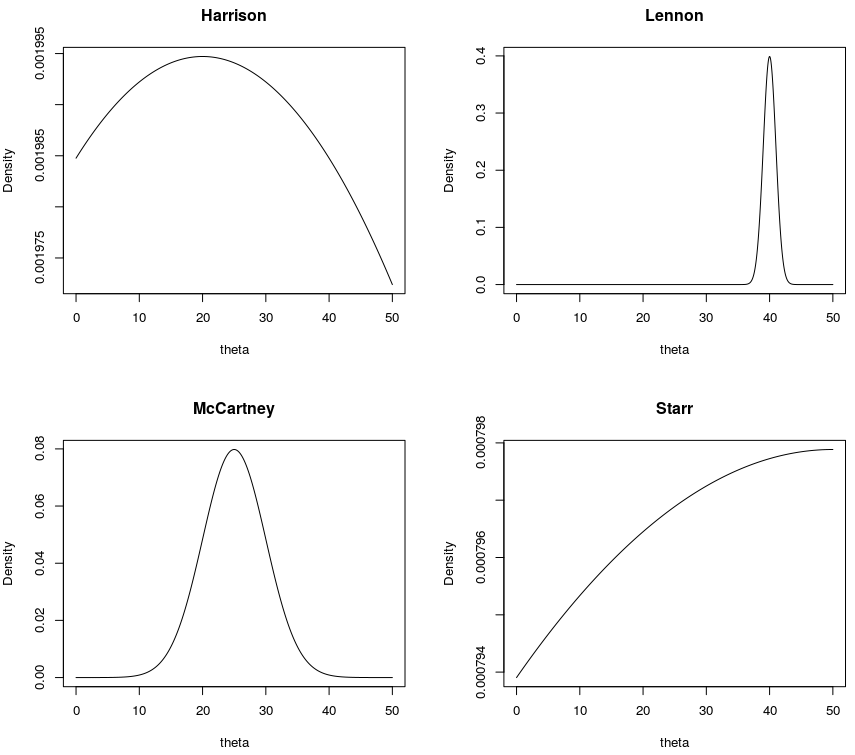
\includegraphics[width=10cm]{Figures/test.png}
                \caption{Posterior distributions for Question C on birds.}
        \end{figure}

        Discuss which prior might be more suitable in the case where: (i) you have little idea on what to expect
        in this new island for your parameter or (ii) expect that the beak width is comparable to what known
        in the previous island (as in Question A).
        Discuss one point for each posterior (e.g. who is the most or least confident, who uses a safest or
        bravest prior, etc ect.).

	\paragraph{Question D}

        You want to study another character, the beak length $\theta_2$ which is correlated with
        the beak width, now labelled $\theta_1$. Your vector of parameters is now
        $\vec{\theta}=\{\theta_1, \theta_2\}$.
        You choose a uniform prior (not conjugate to the Normal distrbution) and therefore choose
        an MCMC algorithm (specifically the Metropolis algorithm) to obtain samples from the
        posterior distribution.

        The algorithm begins by proposing a \textit{proposal} symmetric density
        $q(\vec{\theta}^* | \vec{\theta}^{(t-1)})$ which satisfies
        $q(\vec{\theta}^* | \vec{\theta}^{(t-1)})=q(\vec{\theta}^{(t-1)} | \vec{\theta}^*)$.
        From a starting value $\vec{\theta^{(0)}}$ at iteration $t=0$, for $(t=1,..., T)$
        the algorithm repeats:
        \begin{enumerate}
                \item draw $\vec{\theta}^* = q( \cdot | \vec{\theta}^{(t-1)})$,
                \item calculate $r=h(\vec{\theta}^*)/h(\vec{\theta}^{(t-1)})$,
                \item if $r \geq 1$, set $\vec{\theta}^{(t)}=\vec{\theta}^*$, otherwise\\
                        set $\vec{\theta}^{(t)}=\vec{\theta}^*$ with probability $r$ or\\
                        set $\vec{\theta}^{(t)}=\vec{\theta}^{(t-1)}$ with probability $1-r$.
        \end{enumerate}
        Under mild assumptions, $\vec{\theta}^{(t)}$ converges in distribution to a draw
        from the true posterior density $p(\vec{\theta}|\vec{y})$.

        The samples obtained by this algorithm are auto-correlated, as the sampling at time $t$
        is conditional to the sampling at time $t-1$.
        This is often not entirely satisfactory as ideally we want to draw uncorrelated samples from the
        posterior distribution.
        Propose a modification of the algorithm written above (or write a pseudocode) to ensure that your
        samplings from the Markov chain are fairly uncorrelated.
        Discuss pros and cons of your modification.

 	Another issue in this computation is that $\theta_1$ and $\theta_2$ are highly correlated (or
        you expect them to be highly correlated).
        In this case the chain will have a "slow mixing" and may explore only a fraction of the parameter
        space.
        Propose a modification of the algorithm written above (or write a pseudocode) to ensure that
        you reach convergence (by exploring the whole parameter space) even for correlated parameters
        $\theta_1$ and $\theta_2$.
        Discuss pros and cons of your modification and suggest a computational technique to overcome
        a potential disadvantage of this modification (hint: assume you can use the HPC).







